\documentclass[../summary.tex]{subfiles}

\begin{document}
	
	\section{Economics for sustainability}
	
	\subsection{Study guide}
	
	The study guide for chapter 10 of the MOOC was a complete mess. That is why, even though this part of the summary is still based on the study guide, there won't be a structured overview of it in this summary.
	\\\\
	Typical questions for this chapter are:
	\begin{itemize}
		\item Definitions, terminology: be able to explain the definition, give examples
		\item Graphs: be able to explain and interpret the graphs
		\item Principles: be able to explain, give examples
	\end{itemize}
	
	\subsection{Gross Domestic Product}
	
	The \textbf{Gross Domestic Product} or \textbf{GDP} is a measure of total production that is used to reflect the economic health of a country or region and has strongly increased since the end of the 19th century. Figure \ref{fig:GDP} shows this exponential growth.
		
	\begin{figure}[htbp]
		\centering
		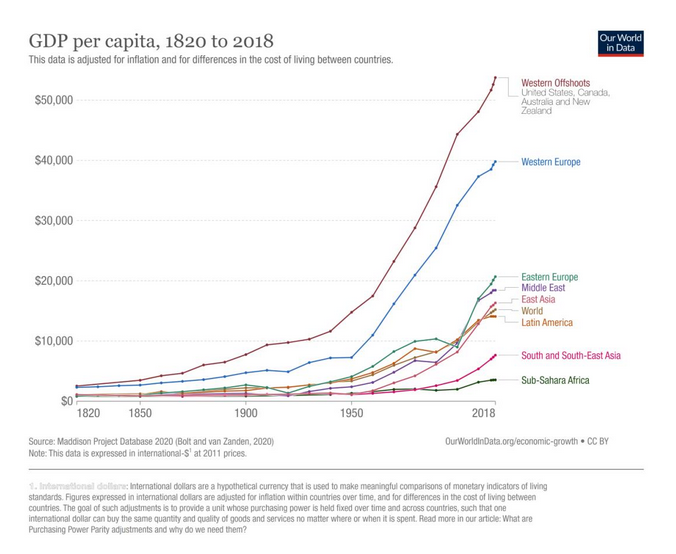
\includegraphics[width=1\linewidth]{images/10-GDP-increase.png}
		\caption{Increase in GDP since 19th century}
		\label{fig:GDP}
	\end{figure}
	
	\newpage
	This increase in GDP went together with a lot of other positive phenomena, such as an increase in life expectancy, an increase in literacy, a decrease in hunger, and so on. However, at the same time, we also saw a rise in environmental pressures, such as greenhouse gas emissions, global warming, plastic pollution, declining biodiversity, and many more. 
	\\\\
	\textbf{Economic growth} is the annual percentage change of real GDP. Real GDP means it's GDP measured in monetary terms but it's corrected for inflation and price changes.
	\\\\
	There are multiple ways to define GDP. The first approach is the so-called \textbf{added value approach}. We define GDP as the value of all final goods and services that are produced in a given country in a given period of time. A second way to define GDP is to look at incomes. All that value added in the GDP is giving rise to incomes, incomes to the persons who own the factors of production. Factors of production are labour, capital and land. So in the second approach to GDP, the \textbf{income approach}, GDP can be defined as the sum of all the incomes that are earned by the owners of factors of production in a given year, in a given country. 
	\\\\
	We should look at GDP as \textbf{a measure of production and of economic activity}. It was not intended to be a measure of prosperity or well-being or happiness. So \textbf{a lot of things are not picked up by the concept of GDP}. A first example of something that is missing in the GDP is a good idea about the distribution or the inequality. A second thing which is missing from the GDP is unpaid work. A third element that is not included in the GDP are changes in the quality of the environment.
	\\\\	
	Figure \ref{fig:emissions-and-GDP-per-capita} shows the emissions and GDP per capita for the different countries. Looking at the graph, we can see there seems to be an increasing relationship between GDP per capita and emissions per capita. Richer countries, with a higher GDP per capita, have higher emissions per capita. We can also see that the big countries, like China and India, are on an intermediate level of emissions. If we study the evolution of the emissions versus the GDP per capita during the 20th and 21st century, like depicted on Figure \ref{fig:emissions-and-GDP-per-capita-long-term}, we notice two different trends. Countries like China and India started at a low level of both emissions and GDP per capita, but they gradually increased over time and are still increasing. On the other hand, we have countries like Belgium and the United States that started increasing at an intermediate level of emissions per capita, but then reached a peak and started decreasing. This pattern is observed for many developed economies and the idea behind it is the so-called Kuznets curve
	
	\begin{figure}[htbp]
		\centering
		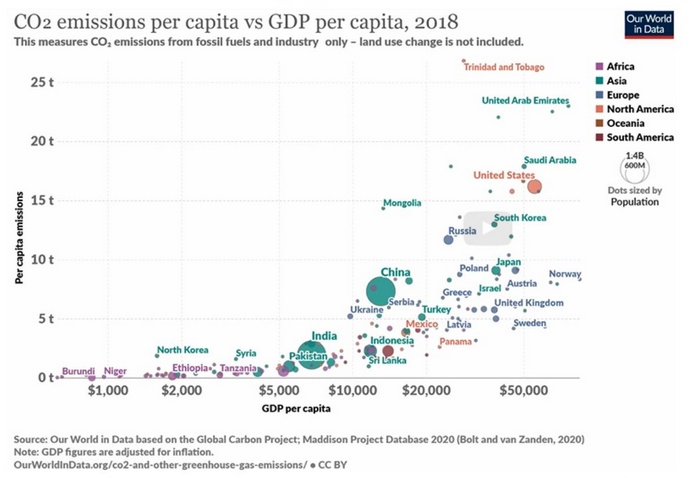
\includegraphics[width=0.9\linewidth]{images/10-emissions-and-GDP-per-capita.png}
		\caption{$CO_{2}$ emissions per capita versus GDP per capita, 2018}
		\label{fig:emissions-and-GDP-per-capita}
	\end{figure}
	
	\begin{figure}[htbp]
		\centering
		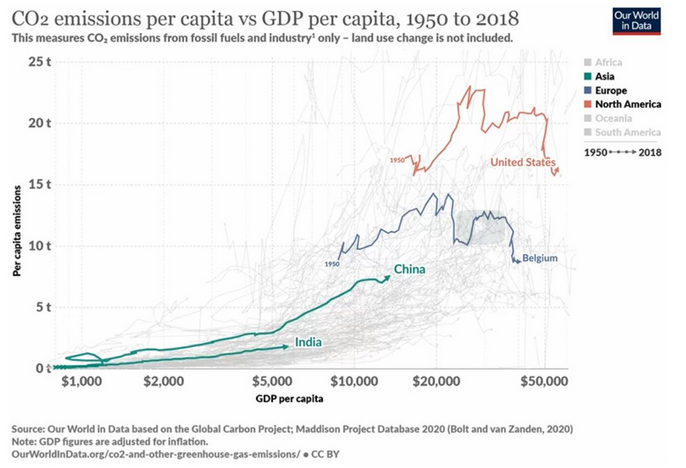
\includegraphics[width=0.9\linewidth]{images/10-emissions-and-GDP-per-capita-long-term.png}
		\caption{$CO_{2}$ emissions per capita versus GDP per capita, 1950 to 2018}
		\label{fig:emissions-and-GDP-per-capita-long-term}
	\end{figure}

	\subsection{The Kuznets curve}
	
	 Like we mentioned in the previous section, the \textbf{Kuznets curve} is used to describe the pattern we see in the evolution of emissions and GDP per capita for countries with developed economies. The Kuznets curve is typically an inverted U-shape of form (Figure \ref{fig:emissions-and-GDP-per-capita-long-term}), meaning that initially countries have very low emissions per capita and GDP per capita. But then they start to economically develop and they start to industrialize. During that industrialization phase, we see rapidly increasing emissions in per capita terms, but also rapidly increasing GDP per capita. At a certain time, there typically comes a moment when economies start to shift away from this heavy industry towards other activities, like, for instance, services. This means that the emission intensity of that economy is gradually decreasing and the growth of their emissions is also decreasing. This can also be influenced by governments that are stepping in and are developing environmental policies to combat pollution. This evolution of first \textbf{increasing, peaking and then decreasing emissions}, that is what we call the Kuznets curve. 
	 \\\\
	 However, it is important to note that this curve is a correlation, and not a causal relationship. Hence, we can't just simply say that the low-income countries just need to focus on growth in order to solve the solution problems.
	 \newpage
	\subsection{Production versus consumption based emissions}
	
	We can make a distinction between production and consumption based emissions. Up until this moment, we have been looking at emissions in the production perspective. \textbf{Production perspective emissions} are a measure of emissions within a given territory of a particular country. However, this is not the full story because we are not only consuming goods that are produced in our country but are also consuming goods imported from other economies. The emissions of these imported goods are not considered in the production perspective we have used so far. If we want to get a fairer approach of our emissions, we should also consider this. This is done by the \textbf{consumption perspective}.
	\\\\
	If we look at our country, we can see that the consumption based emissions are very high. The production based emissions of Belgium are intermediate. For other (production-based) countries like China, we see the opposite. If we calculate the absolute level of emissions, we get an overview of the actual emissions we are causing. We can call this our \textbf{carbon footprint}.
	
	\subsection{Drivers of environmental impact}
	
	If we want to take a look at the drivers for $CO_{2}$ emissions, we first start with the \textbf{IPAT relationship}. This relationship says that environmental impact (I) is the product of 3 drivers: population (P), affluence or GDP per capita (A) and technology (T). The product of these 3 drivers gives rise to the environmental impacts. A special case of this IPAT relationship is the \textbf{Kaya decomposition} of greenhouse gas emission evolution. This decomposition makes a more sophisticated distinction between two technological drivers. Hence, it states the $CO_{2}$ emissions can be written as a product of 4 factors.
	\\\\
	Like previously mentioned, the first driver is \textbf{population}. The more people there are, the more goods and services are produced and the more $CO_{2}$ will be produced. 
	\\\\
	The second driver is GDP per capita. This is a measure of \textbf{affluence}. When people get richer, they typically demand more goods and services which will also result in a rise of emissions.
	\\\\
	In terms of \textbf{technology}, the Kaya decomposition makes a distinction between energy intensity and $CO_{2}$ intensity of energy production. The \textbf{energy intensity} measures how much energy we need to produce one unit (for example $\$1$) of GDP. Unlike the previous factors, we expect the energy intensity to go down over time because our economy becomes more of a service economy instead of an industrial economy and because of technological progress. \\\\
	The \textbf{$CO_{2}$ intensity of energy production} measures how much $CO_{2}$ is released by producing one unit of energy. Since we are currently decarbonizing our energy production by investing in solar panels and wind energy, we also expect this to go down over time.
	\\\\
	Figure \ref{fig:Kaya-decomposition-world} shows the actual global reality of these different factors and their evolution. We can see that the emissions and the GDP grow at the same percentage rate, so there is no decoupling between them. If we look at this evolution for Belgium, we can see that this is not the case. For Belgium, the curves are separating and there is \textbf{absolute decoupling}: whereas on the one hand GDP per capita is still growing, we see that emissions are going down in absolute amount. A \textbf{relative decoupling} would mean that emissions are growing but at a slower pace than the GDP per capita. When we look at the different Kaya factors, we see the same trend as described before for the global overview, with one difference: our population is growing a lot slower than the global population. This results in slightly decreasing $CO_{2}$ emissions since 1990. We can see this in Figure \ref{fig:kaya-decomposition-belgium}.
	
	\begin{figure}[htbp]
		\centering
		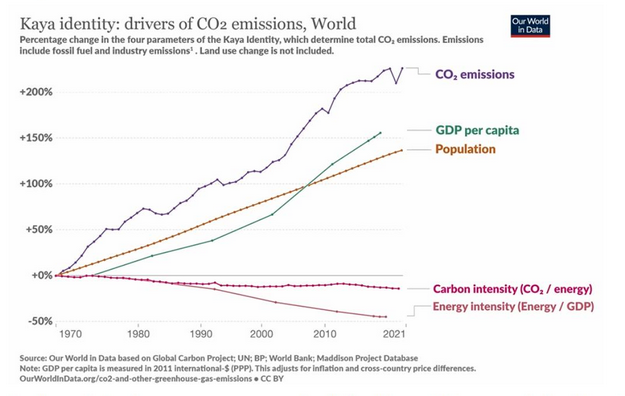
\includegraphics[width=1\linewidth]{images/10-kaya-decomposition-worldwide.png}
		\caption{Kaya decomposition (worldwide)}
		\label{fig:Kaya-decomposition-world}
	\end{figure}
	
	\begin{figure}[htbp]
		\centering
		\includegraphics[width=1\linewidth]{images/10-Kaya-decomposition-belgium.png}
		\caption{Kaya decomposition (Belgium)}
		\label{fig:kaya-decomposition-belgium}
	\end{figure}
	\newpage
	\subsection{Frameworks of sustainable development}
	
	Brundtland defines \textbf{sustainable development} as a development that meets the needs of the present generation without compromising the ability of future generations to meet their own needs. In order to make the concept of sustainable development more operational, we will make a distinction between so-called weak and strong sustainability. But before we do this, we will first introduce the \textbf{different types of capital in economics}.
	\\\\
	 A first concept of capital is \textbf{physical capital}. This type of capital is the physical infrastructure (roads, bridges, ports, canals, but also data networks and so on).
	 \\\\
	 The second type of capital in economics stems from labour, specifically the number of people and their skills. We call this \textbf{human capital}.
	 \\\\
	 Furthermore, there is also the \textbf{natural capital}. This type of capital is generally linked with our renewable and non-renewable sources and level of pollution.
	 \\\\
	 Lastly, we also consider the institutional or \textbf{social capital}. This is about the institutions, police, legal system, judges and so on in a society.
	 \\\\
	 Now, we are able to define \textbf{weak sustainability}. A development path is called weakly sustainable if the total sum of natural, human, physical and social capital is not decreasing over time. If you use a weak concept of sustainability, then you basically allow for substitution between different compartments of capital. For example, it's possible that your natural capital is decreasing, but over-compensated by an increase in another capital stock.
	 \\\\
	 In \textbf{strong sustainability} we require that each of the four capital stocks on their own are non-decreasing over time. So in that case it's not possible anymore that a decrease in one would be compensated by an increase in another capital stock. All of them have to be non-decreasing over time and there can be no erosion.
	 \\\\
	 A first practical example of sustainable development is the \textbf{Adjusted Net Savings} by the World Bank. This concept tracks the evolution of different capital stocks over time on a country level. They make a distinction between the changes in physical, natural and human capital and then make the sum of these changes. If that total sum is positive, we can say that the adjusted net savings are positive and that this country is on a sustainable development track. Clearly, this is an example of a weak sustainability concept because we add the changes in the different capital stocks together. So a decrease in one can be compensated by an increase in another one.
	 \\\\
	 Another example is the \textbf{donut economy concept} of Kate Raworth. This concept is visualised on Figure \ref{fig:donut-economy} and will be explained more detailed in Chapter 11. The outer ring is the environmental sustainability. The economy should not grow out of this environmental safe operating zone. The inner circle refers to the social aspect of the society and the justice elements. Society should not infringe upon the rights and the social and the justice needs of all the members of our society. Hence, this band basically defines the safe and the just space for society to operate in. Looking at the outer ring, we can clearly here see an example of strong sustainability, because this concept is about the safe operating zone in different compartments - biodiversity, climate change and so on - that the society should respect. So here we have an example of a concept that does not allow for trespassing the safe operating zone, and also it does not allow for compensation between the different types of capital in the society. 
	
\end{document}